\section{ARP Who-Has Response}

Address Resolution Protocol (ARP) is used to facilitate mapping
between layer 2 (ethernet) and layer 3 (IP) addresses. When a client
wishes to send a packet to the Soma Backplane (knowing its IP address)
it issues an ARP who-has query to find out the backplane's MAC
address. We respond to this query with our MAC address using this
module.

\subsection{Implementation}
\begin{figure}
\begin{centering}
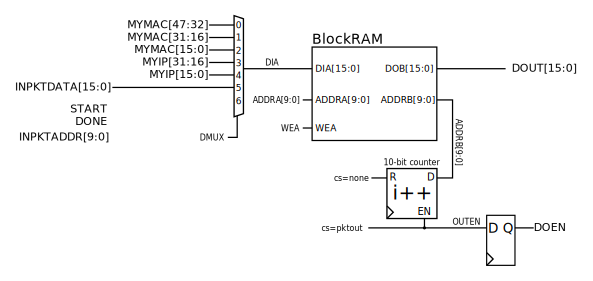
\includegraphics[scale=0.8]{arpresponse.svg}
\end{centering}
\caption{ARP response packet processing module}
\label{arpresponse}
\end{figure}

\begin{figure}
\begin{centering}
\includegraphics[scale=0.8]{arpresponse.fsm.svg}
\end{centering}
\caption{ARP response FSM}
\label{arpresponse.fsm}
\end{figure}



The structure of this module is similar to the ICMP-echo-response
packet processing module. Variable values are written to a ROM. I
really should say more about this.
